%&pdflatex
\documentclass[10pt,border=5pt]{standalone}
\usepackage[utf8]{inputenc}
\usepackage[T2A]{fontenc}

\usepackage{tikz}
\usetikzlibrary{arrows, math, decorations.pathreplacing, calc}

\tikzset{
    >=latex',
    interface/.style={blue, very thick},
    boundary/.style={interface, postaction={draw, decorate, thick,
        decoration={border, angle=#1, amplitude=0.3cm, segment length=2mm, pre length=1mm}}},
    ghost/.style={fill=gray!50},
    eqref/.style={red},
	mapping/.style={eqref, dashed},
    bolddot/.style={shape=circle, fill=black, scale=0.5},
}

\begin{document}
\begin{tabular}{@{}c@{}}

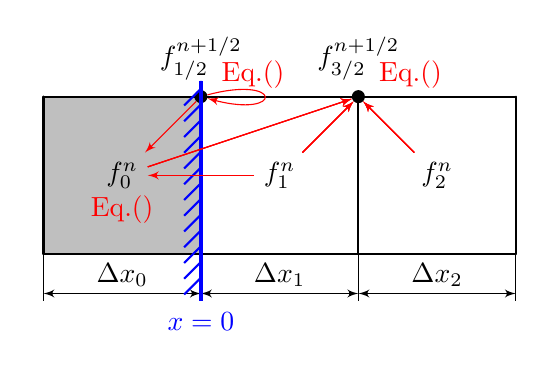
\begin{tikzpicture}
    \fill[ghost] (-2,2) -- (0,2) -- (0,0) -- (-2,0) -- cycle;
    \draw[thick, line cap=round, step=2] (-2,0) grid (4,2);
    \foreach \i [evaluate={\x=\i-1}] in {1,3}
        \node[bolddot, label=above:$f^{n+1/2}_{\i/2}$] (F\i) at (\x,2) {};
    \foreach \i [evaluate={\x=2*\i-1}, evaluate={\a=2*(\i-1)}, evaluate={\b=2*\i}] in {0,1,2} {
        \node (f\i) at (\x,1) {$f^n_{\i}$};
        \draw[<->] (\a,-.5) -- (\b,-.5) node[above=-1pt, pos=0.5] {$\Delta{x}_{\i}$};
    };
    \foreach \x in {-2,0,2,4} \draw (\x,0) -- (\x,-.6);
    \draw[boundary=-45](0,2.2) -- (0,-.6) node[below] {$x=0$};
    \foreach \i [] in {0,1,2}
    \foreach \n in {f0,f1,f2} \draw[->, eqref] (\n) -- (F3);
    \foreach \n in {F1,f1} \draw[->, eqref] (\n) -- (f0);
    \draw[eqref,->] (F1) to [loop right, scale=2] (F1);
    \node at (f0) [eqref, below=4pt] {Eq.()};
    \node at (F1) [eqref, above=8pt, right=4pt] {Eq.()};
    \node at (F3) [eqref, above=8pt, right=4pt] {Eq.()};
    \useasboundingbox (-2.2,-1.1) rectangle (4.2,2.8);
\end{tikzpicture}
\begin{tikzpicture}
    \node {...};
    \useasboundingbox (-0.1,-2.1) rectangle (0.1,1.8);
\end{tikzpicture}
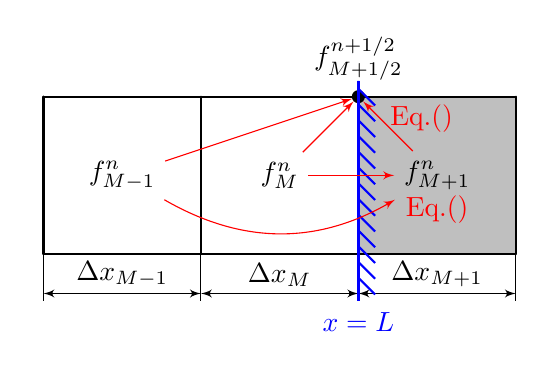
\begin{tikzpicture}
    \fill[ghost] (0,2) -- (2,2) -- (2,0) -- (0,0) -- cycle;
    \draw[thick, line cap=round, step=2] (-4,0) grid (2,2);
    \node[bolddot, label=above:$f^{n+1/2}_{M+1/2}$] (F) at (0,2) {};
    \foreach \idx/\i [evaluate={\x=2*\i-1}, evaluate={\a=2*(\i-1)}, evaluate={\b=2*\i}] in {M-1/-1,M/0,M+1/1} {
        \node (f\i) at (\x,1) {$f^n_{\idx}$};
        \draw[<->] (\a,-.5) -- (\b,-.5) node[above=-1pt, pos=0.5] {$\Delta{x}_{\idx}$};
    };
    \foreach \x in {-4,-2,0,2} \draw (\x,0) -- (\x,-.6);
    \draw[boundary=45](0,2.2) -- (0,-.6) node[below] {$x=L$};
    \foreach \n in {f-1,f0,f1} \draw[->, eqref] (\n) -- (F);
    \draw[->, eqref] (f-1) to[bend right] (f1);
    \draw[->, eqref] (f0) -- (f1);
    \node at (f1) [eqref, below=4pt] {Eq.()};
    \node at (F) [eqref, below=8pt, right=8pt] {Eq.()};
    \useasboundingbox (-4.2,-1.1) rectangle (2.2,2.8);
\end{tikzpicture}
\\
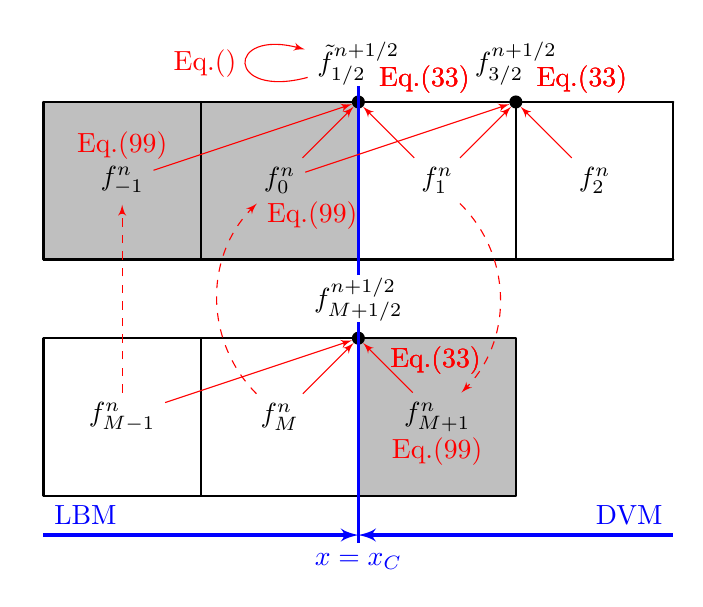
\begin{tikzpicture}
    \fill[ghost] (-4,2) -- (0,2) -- (0,0) -- (-4,0) -- cycle;
    \fill[ghost] (0,-1) -- (2,-1) -- (2,-3) -- (0,-3) -- cycle;
    \draw[thick, line cap=round, step=2] (-4,0) grid (4,2);
    \draw[thick, line cap=round, step=2, yshift=1cm] (-4,-4) grid (2,-2);
    \node[bolddot] (F_DV) at (0,2) {};
    \node[above] (F) at (F_DV.north) {$\tilde{f}^{n+1/2}_{1/2}$} edge [eqref, loop left] node {Eq.()} ();
    \node[bolddot, label=above:$f^{n+1/2}_{3/2}$] (F_DV3) at (2,2) {};
    \node[bolddot, label=above:$f^{n+1/2}_{M+1/2}$] (F_LB) at (0,-1) {};
    \foreach \idx\i [evaluate={\x=2*\i-1}] in {M-1/-1,M/0,M+1/1} {
        \node (f_DV\i) at (\x,1) {$f^n_{\i}$};
        \node (f_LB\i) at (\x,-2) {$f^n_{\idx}$};
    };
    \node (f_DV2) at (3,1) {$f^n_2$};
    \draw[interface](0,2.2) -- (0,-0.2);
    \draw[interface](0,-.8) -- (0,-3.6) node[below] {$x=x_C$};
    \draw[->, interface] (-4,-3.5) node[above right] {LBM} -- (0,-3.5);
    \draw[<-, interface] (0,-3.5) -- (4,-3.5) node[above left] {DVM};
    \foreach \m in {LB,DV} \foreach \n in {f_\m-1,f_\m0,f_\m1} {
        \draw[->, eqref] (\n) -- (F_\m);
    }
    \foreach \m in {LB} \foreach \n in {f_\m-1,f_\m0,f_\m1} {
        \node at (F_\m) [eqref, below=8pt, right=8pt] {Eq.(33)};
    }
    \foreach \m in {DV} \foreach \n in {f_\m-1,f_\m0,f_\m1} {
        \node at (F_\m) [eqref, above=8pt, right=4pt] {Eq.(33)};
    }
    \foreach \m in {DV} \foreach \n in {f_\m0,f_\m1,f_\m2} {
        \draw[->, eqref] (\n) -- (F_\m3);
        \node at (F_\m3) [eqref, above=8pt, right=4pt] {Eq.(33)};
    }
	\draw[->, mapping] (f_LB-1) -- (f_DV-1);
	\foreach \a/\b in {LB0/DV0,DV1/LB1}
		\draw[->, mapping] (f_\a) to[bend left=45] (f_\b);
    \foreach \n/\side/\offset in {f_DV-1/above/0,f_DV0.west/below right/1mm, f_LB1/below/0}
        \node at ($(\n) - (\offset,0)$) [eqref, \side=4pt] {Eq.(99)};
    \useasboundingbox (-4.2,-1.1) rectangle (2.2,2.8);
\end{tikzpicture}

\end{tabular}
\end{document}
